% 3rd - Recognition
%% Includes: Alignment methods, matching, descriptors, hypothesis verification

\chapter{Sparse feature matching}
\label{cha:feature}

% Good intro can be found in Wikipedia SIFT

Solutions to problem stated in section \ref{sec:problem} are commonly divided \cite{something} into feature-based and template-based. The former approach, also referred to as local matching, is focused on comparing point neighbourhoods between the scene and model datasets. 

The solution in such methods is composed of several steps. Firstly, an input subset with elements of rich and distinguishable neighbourhood information is selected. Points that belong to this subset are referred to as \textit{keypoints}. For each keypoint, its neighbourhood information is expressed in the form of a \textit{descriptor} vector. By the means of selected metric, commonly the $L_2$ norm, descriptors are further compared between the scene and model datasets, to find \textit{correspondences} with minimal distance. Such point pairs are then grouped to share similar geometric constrains and finally, the largest clusters are used to calculate affine transformation, which renders the initial problem solution.

The inherent locality of feature matching methods has direct implications on the solution performance. Such methods are by design robust to occlusions \cite{something}. Each point is processed independently, which enables data parallelization to boost time performance. Conversely, keypoint identification requires costly analysis of the whole input dataset, thus a balance between the recognition performance and time effectiveness is required \cite{somethin} for real-time applications.

%---------------------------------------------------------------------------

\section{Shape description} %SHOT}
\label{sec:shape} %shot}

There is a multitude of proposals for shape key-point detectors existing in literature. An overview and performance evaluation of the most popular methods can be found in \cite{keypoints1} and \cite{keypoints2}. From both evaluations, the \textit{Intrinsic Shape Signatures} (ISS) \cite{ISS} detecor is worth particular attention. \cite{keypoints1} states that ISS, as a fixed-scale detector, copes well with full three-dimensional models and provides a proper balance between the repeatability rate and time efficiency. In \cite{keypoints2}, the ISS is evaluated with the best repeatability rate among detector implementations available in PCL. The ISS introduces a saliency measure, defined by the smallest eigenvalue of the neighbourhood scatter matrix. For a given point $p$ and its neighbourhood $N$, the scatter matrix $\Sigma$ is given by
\begin{equation}
\label{eq:scatter}
\Sigma(p,N) = \frac{1}{|N|} \sum\limits_{q\in N}(q -\mu_p)(q - \mu_p)^T,\ \mu_p = \frac{1}{|N|}\sum\limits_{q\in N}q
\end{equation}
% originally defined as weighted matrix, need to check how its implemented
By denoting the eigenvalues of $\Sigma(p, N)$ as $\lambda_1 > \lambda_2 > \lambda_3$, the ISS detector classifies $p$ as a keypoint, if the following condition is satisfied
\begin{equation}
\label{iss}
\frac{\lambda_2}{\lambda_1} < \epsilon_1 \  \land \  \frac{\lambda_3}{\lambda_2} < \epsilon_2 \ \land \  \lambda_3 > \epsilon_3.
\end{equation} 
Thresholds $\epsilon_1$ and $\epsilon_2$ are meant to provide sufficient difference between variations along each principal direction, which aids in estimation of a repeatable reference frames for further description stages. The third threshold $\epsilon_3$ ensures that the variations are large enough to consider the point as interesting. A further improvement to the ISS detection criteria is to apply non-maximum suppression over the saliency measure computed at each point. With this edge thinning technique, a point is classified as a keypoint, if it has the largest $l_3$ over its neighbourhood.  An example of keypoints detected with ISS is presented on figure \ref{fig:iss}. The object (cleaning spray in the center of the figure) has marked points in areas of rich shape information, like the bottleneck or the nozzle. It is also visible, that ISS classifies wrong points in two cases. Firstly, when a point lies on a visibility boundary (i.e. the edges of flat surfaces in the figure), thus it should be extended with boundary detection as described in xx. Secondly, when the sensor noise is high (distant wall flat surface in upper left edge of the figure). This issue can be handled by ignoring points above certain z-distance from the sensor or by adaptatively selecting neighbourhood radius for saliency measure.
%select rich shape object from willow = 13
%implement hardload and iss, measure avg time
%implement in cuda

\begin{figure}[h]
\centering
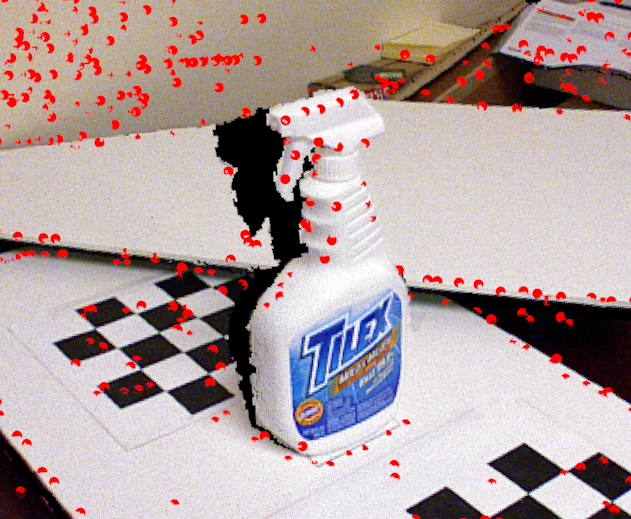
\includegraphics[width=0.8\textwidth]{fig/ISS}
\caption{ISS keypoints (marked with red) computed with $\epsilon_1 =  \epsilon_2 = 0.75$ and $\epsilon_3 = 0.0005$ }
\label{fig:iss}
\end{figure}

The overall time complexity of ISS classification is at the order of $O(nk)$, where $n$ is the image size and $k$ is the max neighbourhood size. This translates into average execution times on target platforms, provided in table \ref{tab:issexec}.

\textit{the ISS method with boundary point re-
moval (ISS-BR) was used to detect the keypoints in the
scene and the models. As reported in (Salti et al, 2012),
ISS achieves the best performance compared to other
keypoint detectors when used in conjunction with fea-
ture descriptors.}

\begin{table}[h]
\centering
\begin{tabular}{r || c | c}
& NVidia Jetson TK1 & Lenovo Y50-70 \\
 \hline
 \hline
 PCL ISS& 4s & 4s \\
 PCL ISSBD& 4s &  4s \\
 CUDA ISS& 4s & 4s \\
 CUDA ISSBD& 4s & 4s
\end{tabular}
\caption{ISS detector time performance statistics.}
\label{tab:issexec}
\end{table}

It is important to note, that in practical applications the keypoint detection step is often replaced by volumetric down sampling. About voxel grid. Model is densely grained. This avoids computational costs of keypoint detection, but increases the complexity of further matching and clustering stages. How to choose this tradeoff.
%In \cite{keypoints-learning}, authors propose a random-forest classifier to be trained for detection of the best interest points for any chosen descriptor.

%Provide complexity, measure time perf (and invariance to transformations?). Can be skipped with uniform.

%A descriptor is considered to be reliable if it is able to capture the same surface characteristics, regardless of rigid transformations, varying sampling density and noise.

Similarly to keypoint detection methods, the literature also abounds with different keypoint description proposals. A comprehensive comparison of the most common methods can be found in \cite{descriptorsComparison}. The \textit{Fast Point Feature Histograms} (FPFH) \cite{FPFH, FPFH2} and \textit{Signature of Histograms of OrienTations} (SHOT) \cite{SHOT} descriptors are particularly interesting for the purposes of this work, given the real-time execution assumptions.


FPFH represents the relative orientation of normal vectors between the query point $p$ and each of its neighbours $q \in N$. For each point pair $(p, q)$, a new coordinate frame $u,v,w$ originating at $p$ is constructed as
\begin{equation}
u = n,\  v = n \times \frac{p-q}{\|p-q\|_2},\  w = u \times v,
\end{equation}
where $n$ is the normal vector at $p$ and $d = \|p-q\|_2$ is the Euclidean distance. Using this reference frame, the difference between normals at $p$ and $q$ is expressed by the angular features
\begin{equation}
\alpha = v \cdot n, \  \phi = u \cdot \frac{(p-q)}{\|p-q\|_2}, \ \theta = \arctan(w\cdot n, u \cdot n).
\label{eq:fpfhangulars}
\end{equation}
The angular features are further binned into a histogram $H$, typically dividing them into $5$ subdivisions, which leads to $3^5=125$ bins. WRONG! FPFHs are decorrelated, 11binned = 33bins. Such histograms are computed every point in the input point cloud. Finally, the FPFH descriptor is formed as
\begin{equation}
FPFH(p) = H(p) + \frac{1}{|N(p)|}\sum\limits_{q\in N(p)}\frac{1}{ \|p-q\|_2}H(q).
\end{equation}
The FPFH descriptor computational complexity is $O(nk)$.


The SHOT proposal emphasises the importance of defining a unique and unambiguous local coordinate system, namely the \textit{Local Reference Frame} (LRF), as a basis for a comparable descriptor construction. A modified version of support covariance matrix (as defined in eq. \ref{eq:scatter}) is introduced, where each neighbour is weighted by its proximity to the query point: 
\begin{equation}
\label{eq:weighCov}
M(p) = \frac{1}{\sum\limits_{q\in N(p)}(r - \|p-q\|_2)} \sum\limits_{q\in N(p)}(r - \|p-q\|_2)(p - q)(p - q)^T.
\end{equation}
The authors determine the LRF coordinate system axes, $x$, $y$ and $z$ with the corresponding eigenvectors of $M$, $e_x$, $e_y$ and $e_z$ in decreasing eigenvalue order. The sign of the axes is disambiguated by aligning the orientation of $x$ and $z$ axes with the majority of vectors they are representing. Concretely, the signed $x$ axis is given by the formula
\begin{equation}
x(p) = \begin{cases}\ e_x, & \mbox{if } \sum\limits_{q \in N(p)} \operatorname{sign}\left( (p-q)^T \cdot x \right) \geq 0 \\ -e_x, & \mbox{otherwise} \end{cases}.
\end{equation}
The $z$ axis sign is determined analogically and $y$ is a cross product of the former, $y = z \times x$. The authors have proven experimentally a high repeatability of such LRF, even in presence of noise and clutter. To form a descriptor, support is further divided with a spherical grid of 2 radial, 2 elevation and 8 azimuth divisions, as depicted on figure \ref{fig:shotgrid} (for better visibility, only half of azmiuth partitions are shown), resulting in 32 cells total.  For each cell, the cosine of the angles $\theta_q$ between the normal at the query point $n_p$ and each normal at cell points $n_q$ are binned to form a histogram. Uniform binning of the cosine function provides robustness to LRF perturbations, as it leads to coarser angle binning for normals close to the $z$ axis. Another problem, called \textit{boundary effect}, arises due to the rough division of the support volume. Depending on the inaccuracies in LRF estimation, points that are close to the boundaries between neighbouring cells are not repeatably accounted to the same histogram. To avoid this problem, the authors propose to interpolate the neighbouring bins to spread the counts among them. After this step, the local histograms are being normalized by their $L_2$ norms, to account for varying point densities. Finally, the SHOT descriptor is composed by concatenating the local histograms, each with typically of 11 bins, resulting in 352 element descriptor.

\usetikzlibrary{3d}

\begin{figure}[ht]
\centering
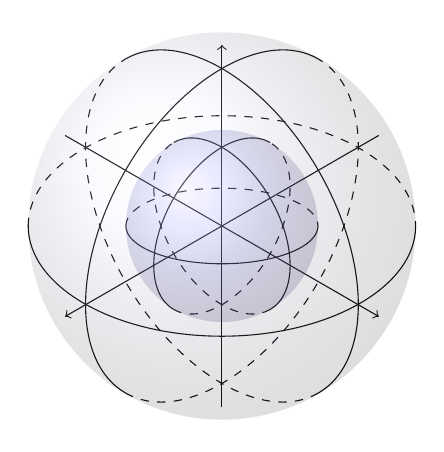
\begin{tikzpicture}[scale=2]
   \begin{scope}[x={(330:1cm)},y={(210:1cm)},z={(90:1cm)}]
    \begin{scope}[canvas is zy plane at x=0]
     \draw (135:1cm) arc (135:-45:1cm);
     \draw[dashed] (135:1cm) arc (135:315:1cm);  
     \draw (135:0.5cm) arc (135:-45:0.5cm);
     \draw[dashed] (135:0.5cm) arc (135:315:0.5cm);   
    \end{scope}
    \begin{scope}[canvas is zx plane at y=0]
     \draw (135:1cm) arc (135:-45:1cm);
     \draw[dashed] (135:1cm) arc (135:315:1cm);
     \draw (135:0.5cm) arc (135:-45:0.5cm);
     \draw[dashed] (135:0.5cm) arc (135:315:0.5cm);   
    \end{scope}
    \draw[->] (0,0,-1.15) -- (0,0,1.15);
    \draw[->] (0,-1.15,0) -- (0,1.15,0);
    \draw[->] (-1.15,0,0) -- (1.15,0,0);
   \end{scope};
   \draw (-1.23,0) arc (180:360:1.23cm and 0.7cm);
   \draw[dashed] (-1.23,0) arc (180:0:1.23cm and 0.7cm);
   \draw (-0.61,0) arc (180:360:0.61cm and 0.24cm);
   \draw[dashed] (-0.61,0) arc (180:0:0.61cm and 0.24cm);

   \shade[ball color=blue!10!white,opacity=0.20] (0,0) circle (1.23cm);
   \shade[ball color=blue!50!white,opacity=0.20] (0,0) circle (0.61cm);
\end{tikzpicture}
\caption{SHOT descriptor spherical grid}
\label{fig:shotgrid}
\end{figure}

%Signatures vs histograms. About SHOT. Complexity, time perf.
Extension with color. \cite{CSHOT}. Performance extension in binarized form \cite{BSHOT}.

%----------------------------	-----------------------------------------------

\section{Texture description} %ORB}
\label{sec:color} %orb}

%TODO
% - add model2views conversion to ros_recognizer
% - test SIFT, SURF and ORB with different RGB2GREY, opponent color
% - 

In addition to the spatial information contained in RGB-D images, an important and discriminative function is performed by the description of texture. Although there are descriptor proposals in literature that combine both modalities \cite{CSHOT, RGBFPFH}, the best matching performance is achieved when color variation is analyzed independently of shape. This is because the key characteristic points typically do not overlap between modalities and separating them benefits in further matching phase, where descriptors of smaller sizes are compared in the same information domain, with overall more keypoints for grouping and generating pose hypotheses.

In comparison to shape, texture descriptors are more broadly studiend and developed field. A significant interest in this area was aided by numerous successful applications \cite{ORB} of the \textit{Scale-invariant Feature Transform} (SIFT) \cite{SIFT}, which defines methods for both interest-point selection and feature description. To achieve scale invariance, SIFT introduces a linear scale-space, defined as a convolution
\begin{equation}
L(x,y,\sigma) = G(x,y,\sigma) \ast I(x,y),
\label{eq:scalelinear}
\end{equation}
where $I(x,y)$ is the input image and $G(x,y,\sigma) = \frac{1}{2\pi\sigma^2}e^{-(x^2 + y^2)/2\sigma^2}$ is a Gaussian function with a scale parameter $\sigma$. Keypoint detection is further based on finding extrema of a \textit{Difference of Gaussian} (DoG) function, given as
\begin{equation}
DoG(x,y,s) = L(x,y,s + \Delta s) - L(x,y,s)
\end{equation}
To account for for strong responses along the edges, DoG extrema are suppressed by a Hessian criterion
\begin{equation}
\frac{\det H}{(\mathrm{trace} H)^2} \geq \frac{r}{(r+1)^2},\ H = \begin{bmatrix}
L_{xx} & L_{xy} \\
L_{yx} & L_{yy} 
\end{bmatrix},
\end{equation}
where $r \geq 1$ is the upper limit imposed on the ratio between largest and the smallest eigenvalues of $H$ \cite{SiftScholarpedia}. An example of a SIFT detected keypoints is presented in fig. \ref{fig:sift}.

\begin{figure}[ht]
\centering
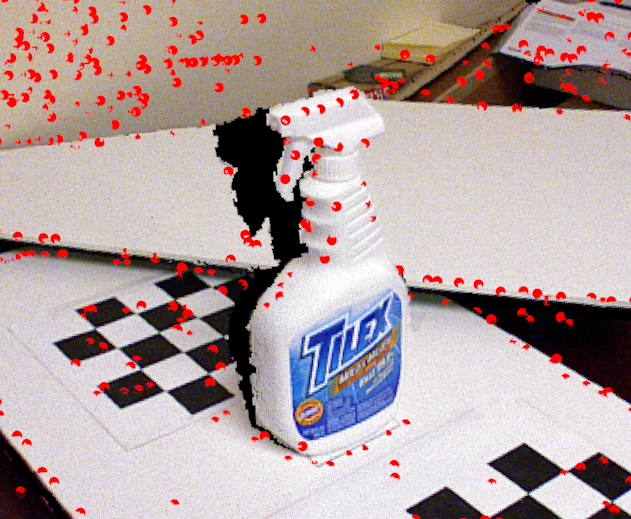
\includegraphics[width=0.8\textwidth]{fig/ISS}
\caption{SIFT keypoints marked with circles. Scale is represented by circle radius}
\label{fig:sift}
\end{figure}

Each selected interest point has a corresponding scale parameter, that is used in further description phase of SIFT to determine the neighbourhood size and achieve scale invariance. The SIFT descriptor has also a ratotational invariance property, which means that rotating the neighbourhood of a query point does not change its descriptor vector. Such invariance is achieved by assigning an \textit{dominant orientation} parameter to each keypoint. Gradient directions, computed from gradient vectors $\Delta L(x,y,s)$ in scaled keypoint neighbourhood are accumulated in a 36-binned histogram. Maximum peak of such histogram renders the dominant orientation.

To form the SIFT descriptor, a 4x4 rectangular grid aligned to the dominant orientation is applied on the keypoint neighbourhood. In each cell, an 8-binned histogram of gradient orientations, also aligned to the dominant direction is computed. The histogram inputs for each gradient are weighted by its magnitude. Histograms for each cell are further concatenated into a single descriptor, which renders 128 dimensions. The final descriptor is normalized to unit sum, to be robust against illumination variations.

TODO: add grid visualization

The \textit{V4R} framework bases its recognition performance on the SIFT descriptor discriminative properties. Concretely, it uses the GPU-accelerated implementation, proposed by \cite{SIFTGPU}. The SIFT, however, is a patented solution \cite{SIFT-PATENT} that requires licence fees for commercial applications. Moreover, its 128 floating point descriptor is costly in both computing and matching phases, even with GPU paralellization. There are several alternatives to SIFT that overcome this drawbacks. This work attempts to extend the V4R framework and evaluate the performance of selected SIFT alternatives.

\textit{Oriented FAST and Rotated BRIEF} (ORB) \cite{ORB} is a particularly interesting proposal, because of its real-time capabilities. As the name suggests, it is an enhancement to a two former concepts, the\textit{ Features from Accelerated Segment Test} (FAST) \cite{FAST} keypoint detector and the \textit{Binary Robust Independent
Elementary Features} (BRIEF) \cite{BRIEF} descriptor.

FAST detector analyses a circle of 16 pixels around the query point and classifies it as a corner, if there are $n$ contiguous pixels with all darker or all brighter intensity by a given threshold. To boost the efficiency of computation, a decision tree is optimized to for the classification task. The authors reported, that $n = 9$ contiguous pixels achieved the best repeatability in the their tests. In ORB, FAST keypoints are ehanced to achieve scale and rotation invariance. Detection is performed across a scale pyramid and an orientation component is introduced, by computing a weighted intensity centroid of the query neighbourhood patch. 

BRIEF descriptor is designed to minimize the CPU and memory footprint. It is defined over an image patch intensity $I_p$ as
\begin{equation}
\mathrm{BRIEF}(I_p) = \sum \limits_{0\leq i < n}2^i\cdot \tau(I(p_i), I(q_i)),\ \tau(x, y) = \begin{cases} 1, & \mbox{if } x < y \\ 0, & \mbox{otherwise} \end{cases}
\end{equation}
where $p_i$, $q_i$ are selected pixel coordinates within the patch, $\tau$ is an intensity test and $n$ is the bitstring size. The authors have experimentally proven that $n=256$ yields an effective compromise between the discriminative performace, computation speed and memory efficiency. Given an image patch of size $S\times S$, the pixel coordinate test pairs $(p_i, q_i)$ are randomly taken from a Gaussian distribution, with $0.04\cdot S^2$ variance for the first pixel location and $0.01\cdot S^2$ for the second. Due to the fact, that $\tau$ compares intensities of single pixels, the image patch has to be smoothened before computing the descriptor to reduce the noise. Gaussian kernel of size $9\times 9$ and variance of 2 was selected to for this task. ORB has different smoothing. They rotate, compute lookup, train uncorrelated with greedy-search.

Similarily to ORB, the \textit{AKAZE} \cite{AKAZE} descriptor is also designed for real-time efficiency. The main characteristic which distinguishes it from the formerly introduced SIFT and ORB, is the non-linear scale space. Despite the strong analytical foundations and wide area of applications for the linear scale theory, its main disadvantage in the context of object recognition, is the fact that it does not preserve edges. Object boundaries and texture characteristics are blurred, which may lead to imprecise matching. The key idea behind AKAZE is to make filtering in the scale pyramid adaptive to local intensity variations and thus preserve the edges in the image. A comparison between the subsequent images of a linear and non-linear scale pyramids is shown in the figure \ref{fig:scalepyramids}

Gaussian scale space given in equation \ref{eq:scalelinear} can be derived as a solution to a diffusion equation
\begin{equation}
\partial_s L = \frac{1}{2}\nabla^2L
\end{equation}
with initial condition $L(x,y,0) = I(x,y)$. This approach is generalized to define a non-linear scale space, as a solution to an anizotropic diffusion equation
\begin{equation}
\partial_s L = \mathrm{div}\left( c(x,y,s) \nabla L \right) = \nabla c \cdot \nabla L + c(x,y,s)\nabla^2L.
\label{eq:nonlindiffusion}
\end{equation}
The \textit{conductivity} function $c$ is designed to achieve the adaptive filtering. The AKAZE authors suggest a function that promotes wider image regions and has the form of
\begin{equation}
c(x,y,s) = \frac{1}{1 + \frac{|\nabla L_{\sigma}|^2}{\lambda^2}},
\end{equation}
where $L_\sigma$ is a gaussian smoothed image luminance and $\lambda$ is a contrast factor, that controls the level of diffusion. AKAZE uses \textit{Fast Explicit Diffusion} algorithm to find an approximate solution to equation \ref{eq:nonlindiffusion} and form the scale pyramid of $O$ octaves and $S$ sublevels. Keypoint detection is further based on finding local maxima of Hessian determinant at each pyramid level. Finally, the \textit{Modified-Local Difference Binary} (M-LDB) descriptor is introduced to represent the local image structure around the keypoint. It is similiar to the previously descibed BRIEF descriptor, in a way that it divides the keypoint neighbourhood into a grid and performs a series of comparisons among the cells to form a binary vector. Hovewer, instead of direct comparison of intensities at each pixel, it performs 3 binary tests over average intensity and the mean horzontal and vertical derivatives. How many bits final ?

It is important to note, that all of the algorithms presented so far in this section operate over greyscale images. The loss of information caused by dimensionality reduction of the RGB color space can lead to performance degradation of the recognition system. In \cite{RGB2GREY}, the authors compare 13 different methods for RGB to gray conversion and conclude the superiority of simple channel-wise average over i.e. using intenisites form other color spaces, like HSV or CIELAB. Color employment for object detection is thoroughly evaluated in \cite{ColorComparison}. The authors have compared results of image classification with SIFT descriptor computed independently over each channel of different color spaces and yield \textit{Opponent-SIFT} and \textit{W-SIFT} as the leading approaches. The first method is based on the biologically inspired \textit{oppoonent} color space, transformed from RGB channels by
\begin{equation}
O_1 = \frac{R - G}{\sqrt{2}},\ O_2 = \frac{R + G - 2B}{\sqrt{6}},\ O_3 = \frac{R + G + B}{\sqrt{3}}.
\end{equation}
The latter approach enhances opponent space by removing influence of light intensity from color channels, defining the invariants as $\frac{O_1}{O_3}$ and $\frac{O_2}{O_3}$. Computing and matching image descriptors on each color channel increases the computational demands, but can be beneficial from recognition rate point of view. The profits of using this approach will be evaluated further in this chapter. Average computation times on target platforms are provided in table \ref{tab:opponent}. Tested implementation from OpenCV with modifications for
%---------------------------------------------------------------------------

\section{Correspondences}
\label{sec:correspondences}

Once the model and input images are described in a comparable manner, a relationship can be set between their keypoints. This is done by the means of a selected distance metric $d$ and a condition (typically a threshold $\tau$ on the distance) to accept a queried scene descriptor as a match to its model nearest neighbour. A set of point pairs, or \textit{correspondences}, is formed this way, from which the object pose is further inferred.

From performance perspective, it is important to note that simply comparing all the features to find all possible matches between images is a quadratic operation in the number of selected keypoints. In real-time applications, this approach, namely \textit{bute-force} matching, is unfeasible for high dimensional feature vectors like SHOT or SIFT. An efficient alternative is to employ an indexing structure \cite{szeliski}, in example a hash-table or a Kd-tree (as described in \ref{sec:neighbourhood}). Search trees are comprehensively evaluated for this purpose in \cite{flann} and multiple randomized Kd-trees are concluded to achieve the best performance.
%TODO: elaborate more from neighbourhood

Despite the complexity optimizations of nearest neighbour search for real valued descriptors, they are still outperformed in matching time by binary descriptors, even with brute-force approach (see table XX). This is because computing the distance metric, i.e. the $L_2$ metric, is far more demanding than applying Hamming distance to binary features of the same dimensionality. The former requires costly floating point operations, while the Hamming distance is computed only with XOR and a bitcount, which is highly optimized on modern computing architectures with SSE instructions \cite{ORB}. Furthermore, in \cite{binaryFlann}, the authors propose a search tree specifically designed for binary features to further boosts the matching performance. Experimental results on the matching performance are provided in table XX.

computation

%---------------------------------------------------------------------------

\section{Clustering}
\label{sec:clustering}

Keypoint correspondences established in the previous step represent only local similarities between the model and the scene. As a result, false matches may occur if a part of the scene, not belonging to the object, resembles locally a part of the model. Furthermore, the scene may contain multiple object instances, thus model keypoints may posess many counterparts in the scene and there may exist true matches with different inferred poses. For these reasons, the relationship between the correspondences has to be considered, in order to discard false matches and group together those that belong to the same object instance. There are three popular methods designed for this purpose: \textit{geometric consistency}, \textit{pose clustering} and \textit{hough voting} \cite{hough}.

The first method is based on the rigid transformation property to preserve distances between point pairs. Geometric consistency \cite{geometricConsistency,multiPipeline} grouping, starts from a seed correspondence $(p_i, q_i)$ and iteratively creates clusters of matches conforming to a distance constraint:
\begin{equation}
\left|\left\Vert p_i - p_j \right\Vert_2 - \left\Vert q_i - q_j \right\Vert_2\right| < \epsilon,
\label{eq:correspondence-constrain}
\end{equation}
where $p$ and $q$ are model and scene keypoints, $i$ and $j$ are correspondence indexes and $\epsilon$ is a tuneable parameter called \textit{consensus set dimension}. Constrain \ref{eq:correspondence-constrain} enforces that the distance between two clustered model points is close to the distance of their corresponding matches within the scene, as depicted on figure \ref{fig:corr-constrain}. By ensuring that clustered corresondences meet rigid transformation requirement, this method imposes a weak condition for presence of a single object instance. Moreover, by providing a threshold of the subset size, a large number of false matches are rejected.

The next approach, introduced in \cite{poseClustering}, requires additional information in the form of a LRF (as described in section \ref{sec:shape}) to be associated with each matched feature. By providing reference frames, rigid transformation can be directly computed from a single pair of corresponding keypoints. Rotation $R \in \mathbb{R}^{3\times 3}$ and translation $t \in \mathbb{R}^3$ are given by
\begin{equation}
R = R_q^T \cdot R_p,\ t = q - R\cdot p,
\label{eq:corr-pose}
\end{equation}
where $p$ and $q$ are model and scene keypoints, and $R_p$, $R_q$ are rotation matrices with rows composed of LRF unit vectors of $p$ and $q$. The authors further propose to convert $R$ into Euler angles (algorithm for conversion is described i.e. in \cite{rotationToEuler}), concatenate the angles with translation, and use the resultant 6-dimensional vectors within a standard k-means clustering algorithm. Similarly to geometric consistency, larger groups of correspondences indicate a single object instance and clusters with size less than a given threshold are then discarded to cope with false matches.

Finally, the last important technique is hough voting. \textit{Hough transform}, initially developed for detecting 2D lines in intensity images, became a widespread method for detecting arbitrary parameterized shapes \cite{generalizedHough}. The key idea of this method is to cast \textit{votes} on parameters from every feature point in the image and gather them in \textit{accumulator} structure. The accumulator is a $N$-dimensional grid over the parameter space, where $N$ is parameter dimensionality. Cells of this grid compose a histogram of votes on parameter values.

In case of correspondence clustering, similarily to the previous method, Hough voting requires each feature to have associated LRF, to compute the pose for every match from eq. \ref{eq:corr-pose}. Using the same parameter space, hovewer, would lead to a sparse, 6-dimensional accumulator grid with computational and memory demands. To overcome this problem, in \cite{hough}, the authors propose to cast votes on the object centroid position, instead of its full 6D pose. Within an offline stage of the algorithm, each keypoint $p$ is associated with model centroid position $c_p$ in LRF coordinate system. During voting stage, each matched scene feature point $q$ transforms this centroid to the scene coordinate system, with
\begin{equation}
c_s = R_q^T \cdot c_p + q,
\end{equation}
where $R_q$ is a rotation matrix composed of LFR unit vectors at $q$. Centroid $c_s$ is used to cast votes over a 3-dimensional accumulator histogram. To account for quantization within the accumulator and the inaccuracy of LRF estimation, each bin is summed with its 6 closest neighbours. Peaks of the histogram that exceed a given threshold are considered to indicate a single object instance.

Quantitative comparison of these three methods impl.

%---------------------------------------------------------------------------

\section{Alignment}
\label{sec:alignment}
 
Having correspondences grouped in clusters, the next step is to estimate a common pose that they represent. Since the constrain from the grouping step apply only to the distance of the matched points, but not their direction, it does not fully discard correspondences not conforming to rigid transformation model (as illustrated in fig. \ref{fig:corr-constrain}). To account for such model \textit{outliers}, a robust estimator \textit{Random Sample Consensus} (RANSAC) \cite{ransacbase} is used to calculate the pose. In its basic form, the RANSAC algorithm is essentially composed of two, iteratively repeated steps \cite{wikipedia,ransacdummies}:
\begin{enumerate}
\item Firstly, a minimal sample subset is randomly selected from the input dataset, that allow for computing the model parameters. In case of rigid transformation, three point pairs are enough for a closed form solution \cite{umeyama}. Give umeyama solution.
%TODO: Give umeyama solution
\item Secondly, the remaining dataset points are tested to be consistent with the model computed in the sampling step. A data point will be considered as an inlier if it fits the computed model within a defined error threshold. The set of such elements is called a consensus set. If the consensus set contains enough points, the model is reestimated from all selected inliers and evaluated with the error of the inliers relative to the model.
\end{enumerate}
This procedure is then repeated until a termination condition is met, which usually is a fixed number of iterations.
%TODO: Find out difference between umeyama and Closed-form solution of absolute orientation using unit quaternions